\documentclass[a4paper,12pt]{report}
\usepackage[utf8]{inputenc}
\usepackage{enumitem}
\usepackage{graphicx} %para las imágenes
\usepackage{float} %para fijar las imágenes
\usepackage{circuitikz} % Para dibujar circuitos
\usepackage[spanish]{babel} % To set title in talbles and figures in spanish 
\usepackage{comment}
\usepackage{amsmath,amssymb,amsfonts}
\usepackage{graphicx}
\usepackage{mathrsfs}
\usepackage{xcolor}
\usepackage{booktabs}  % For professional table formatting
\usepackage{dcolumn}   % For alignment on decimal points
\usepackage{caption}   % For customizing captions
\usepackage{subcaption}
\usepackage{booktabs} % for tables
\usepackage{multirow} % for tables
\usepackage{threeparttable} % for tables
\usepackage[normalem]{ulem} % strikethrough font
\usepackage{pgfplots}
\usepackage{siunitx} %Para poder usar \ohm para el simbolo de ohm
\usepackage{pdfpages}
\usepackage{tabularx}
\usepackage{lastpage}
\usepackage{wrapfig}
\usepackage{minted}
\usepackage{subcaption}
\usepackage{gitdags}
\usepackage[hidelinks]{hyperref}

\newcommand\numeq[1]{(\ref{#1})}
\newcommand\eq[1]{Eq.~(\ref{#1})}
\newcommand\eqs[1]{Eqs.~(\ref{#1})}
\newcommand\fig[1]{Figura~\ref{#1}}
\newcommand\numfig[1]{\ref{#1}}
\newcommand\figs[2]{Figs.~\ref{#1} y~\ref{#2}}
\newcommand\sect[1]{Section~\ref{#1}}
\newcommand\subsect[1]{Subsection~\ref{#1}}
\newcommand\sects[1]{Sections~\ref{#1}}
\newcommand\nsect[1]{\ref{#1}}
\newcommand\apen[1]{Appendix~\ref{#1}}
\newcommand\pag[1]{Page~\pageref{#1}}
\newcommand\bib[1]{\cite{#1}}
\newcommand\tabla[1]{Tabla~\ref{#1}}
\newcommand\tablas[2]{Tablas~\ref{#1} y~\ref{#2}}
\addto\captionsspanish{\renewcommand{\tablename}{Tabla}}


\usepackage[a4paper, %margenes de pagina
  left=2.5cm,
  right=2.5cm,
  top=1cm,
  bottom=2cm,
  includehead
]{geometry}

% Encabezado
\usepackage{fancyhdr}
\pagestyle{fancy}
\cfoot{\thepage}
\setlength{\headwidth}{\textwidth} % Hace que el ancho del encabezado coincida con el ancho del texto
\setlength{\headheight}{15pt}  % Ajusta la altura del encabezado
\setlength{\headsep}{30pt}     % Ajusta la separación entre el encabezado y el contenido

\usepackage{titlesec}
\titleformat{\chapter}[display]
  {\normalfont\LARGE\bfseries}{}{0pt}{}
\titlespacing*{\chapter}{0pt}{-35pt}{10pt}
\usepackage{etoolbox} 
\makeatletter
\patchcmd{\chapter}{\thispagestyle{plain}}{\thispagestyle{fancy}}{}{} %Muestra encabezado en las paginas con \chapter
\makeatother

\makeatletter
\newcommand{\subtitledoc}[1]{\newcommand{\@subtitledoc}{#1}}
\newcommand{\instituto}[1]{\newcommand{\@instituto}{#1}}
\newcommand{\carrera}[1]{\newcommand{\@carrera}{#1}}
\newcommand{\titular}[1]{\newcommand{\@titular}{#1}}
\newcommand{\ayudante}[1]{\newcommand{\@ayudante}{#1}}
\newcommand{\catedra}[1]{\newcommand{\@catedra}{#1}}
\newcommand{\curso}[1]{\newcommand{\@curso}{#1}}
\newcommand{\footerauthor}[1]{\newcommand{\@footerauthor}{#1}}
\newcommand{\numero}{%
  N\textsuperscript{o}%
}

%formato de encabezado y pie para todas las paginas.
\fancyhead[L]{
    \begin{minipage}[b]{7.5mm}
        
\includegraphics[width=12mm]{villada.png}
    \end{minipage}
}
\fancyhead[R]{
    \@title
}
\fancyhead[C]{
    \textbf{\@catedra}
}
\fancyfoot[C]{} %eliminar antiguo numero de pagina
\fancyfoot[R]{Página \thepage\ de \pageref{LastPage}}
\renewcommand{\headrulewidth}{0.5pt}
\renewcommand{\footrulewidth}{0.5pt}
\pagestyle{fancy}

\renewcommand{\contentsname}{Tabla de Contenidos}

\usepackage{afterpage}
\newcommand\myemptypage{
  \newpage
  \null
  \thispagestyle{empty}
  \addtocounter{page}{-1}
  \newpage
}

\renewcommand{\maketitle}{%
    \newpage
    \thispagestyle{empty}
    \begin{center}

    \textsc{\LARGE \@instituto}\\[0.5cm] 
    \textsc{\Large \@carrera}\\[1.5cm] 
    
\includegraphics[width=0.30\textwidth]{villada.png} \par
    \vspace{1.5cm}
    
    {\huge\bfseries \@title}\\[0.4cm]
    \textsc{\Large \@subtitledoc}\\[0.5cm]
    

    \end{center}

    \vspace{2cm}

    {\noindent
    \begin{minipage}[t]{.2\textwidth}
        \raggedright
        \textbf{DOCENTES} \par
        ~\\ \par
        \textbf{CÁTEDRA} \par
        \textbf{CURSO} \par
        \medskip
        \end{minipage}%
        \begin{minipage}[t]{.05\textwidth}
        \raggedright
        \textbf{:} \par
        ~\\ \par
        \textbf{:} \par
        \textbf{:} \par
        \medskip
    \end{minipage}%
    \begin{minipage}[t]{.55\textwidth}
        \raggedright
        \@titular. \par
        \@ayudante. \par
        \@catedra. \par
        \@curso \par
        \medskip
        \@author \par
    \end{minipage}%
    \begin{minipage}[t]{.15\textwidth}
        \raggedright
        ~\\
        ~\\
        ~\\
        \medskip
    \end{minipage}
    }
    \vfill
    \begin{center}
        \textbf{CÓRDOBA, ARGENTINA} \par
        \textbf{\@date}
    \end{center}
    \newpage
}

\makeatother

\begin{document}
\title{Apunte de Git}
\subtitledoc{Control de Versiones}
\instituto{Instituto Técnico Salesiano Villada}
\carrera{Especialidad en Informática}
\titular{Cortesini Perez Luciano Tomas}
\ayudante{Marchisone Mateo}
\catedra{Programación I}
\curso{4to año C}

\maketitle

\chapter{Introducción}
\setcounter{page}{1}
\section{Que es git?}
GIT (Global Information Tracker) es un sistema de
control de versiones distribuido, gratuito y de código
abierto, diseñado para gestionar el historial de cambios
en el código fuente de proyectos de software de forma
rápida y eficiente. Permite a los desarrolladores rastrear
modificaciones, volver a versiones anteriores y trabajar
colaborativamente sin sobrescribir el trabajo de otros.
Git utiliza un modelo basado en instantáneas (snapshots), donde cada confirmación (com-
mit) representa el estado completo del proyecto en un momento determinado.rsión.

Cuando decimos que Git es un sistema de control de versiones \textbf{distribuido}, significa que
cada copia del repositorio contiene el historial completo del proyecto.
No dependemos de un único servidor para trabajar: podemos hacer commits, crear ramas y consultar historial sin conexión.
Si un servidor remoto falla, cualquier copia del repositorio sirve para recuperar la totalidad del contenido.

\section{Que es GitHub?}
\textbf{GitHub} es una plataforma en línea para alojar repositorios Git y colaborar con otras personas.
Permite compartir código, revisar cambios, trabajar en equipo mediante ramas y pull requests, y mantener un respaldo remoto del proyecto.

Es importante distinguirlos: \textbf{Git no es GitHub}.
Git es la herramienta que funciona en nuestra computadora (local), mientras que GitHub es un servicio web que usa Git para facilitar la colaboración y la publicación de repositorios.
Se puede usar Git sin GitHub, y también existen otras plataformas similares (por ejemplo, GitLab o Bitbucket).

\section{Por que usamos git?}
Usar Git y GitHub mejora el flujo de trabajo porque permite:
\begin{itemize}[leftmargin=*]
  \item trabajar con seguridad, ya que los cambios quedan registrados y se pueden deshacer;
  \item experimentar sin perder avances, creando commits frecuentes y ramas;
  \item colaborar de forma ordenada, integrando aportes de varias personas;
  \item mantener respaldo y trazabilidad del proyecto en el tiempo.
\end{itemize}

\chapter{Conceptos Básicos}
\section{Repositorio}
Un repositorio en Git es un directorio que contiene tu proyecto junto con toda su historia: cada
cambio que se hizo, cuándo, quién lo hizo y por qué.
Técnicamente, es una carpeta normal con un subdirectorio oculto llamado .git donde Git guarda toda
esa información. Ese .git es el corazón del repositorio: sin él, sería solo una carpeta común.
Hay dos tipos principales:

\textbf{Local} — vive en tu máquina. Ahí trabajas, hacés commits, creás ramas. Es completamente funcional sin internet.

\textbf{Remoto} — vive en un servidor (GitHub, GitLab, etc.). Sirve como punto central para compartir el trabajo con otros o como respaldo.

\section{Commit}
Un commit es una instantánea (foto) del estado de tu proyecto en un momento dado, guardada permanentemente
en la historia del repositorio.
Cada vez que hacés git commit, Git toma todos los cambios que preparaste (los que están en el staging area) y
los congela en un paquete inmutable que incluye:

\begin{itemize}
  \item \textbf{El contenido} — cómo quedaron los archivos en ese momento.
  \item \textbf{Metadatos} — autor, fecha y hora.
  \item \textbf{Mensaje} — descripción de qué cambió y por qué.
  \item \textbf{Referencia al commit anterior} — así se forma la cadena de historia.
\end{itemize}

Esa cadena es clave: cada commit apunta al que lo precedió, formando una línea de tiempo que podés
recorrer hacia atrás en cualquier momento.

\begin{figure}[h]
  \centering
  \begin{tikzpicture}[scale=1.5, transform shape]
    % Commit DAG
    \gitDAG[grow right sep = 2em]{
      A -- B -- C
    };
  \end{tikzpicture}
  \label{fig:commit_dag}
  \caption{Linea de tiempo de commits}
\end{figure}

En la Figura~\ref{fig:commit_dag} se muestra una secuencia de commits A, B y C, donde cada uno apunta
al anterior, formando una historia lineal del proyecto.

Un commit es como el botón de guardar partida en un videojuego. No solo guardás
el progreso actual, sino que podés tener múltiples puntos de guardado y volver exactamente a
cualquiera de ellos si algo sale mal.


Git identifica cada commit con un hash SHA-1, un código único como a3f4c91....
Ese hash es calculado a partir del contenido del commit, de este modo git garantiza que el contenido
no fue corrompido o alterado, lo que hace a los commits confiables e inmutables. \\

El mensaje o \textbf{commit message} debe describir de forma clara qué se cambió y por qué.
Buenas prácticas recomendadas:
\begin{itemize}
  \item usar frases breves y concretas;
  \item escribir en imperativo (por ejemplo: ``Agrega README.md'');
  \item evitar mensajes genéricos como ``cambios'' o ``arreglos'';
  \item si hace falta, agregar una descripción más larga explicando contexto.
\end{itemize}


\section{Áreas de un proyecto Git}
El flujo de trabajo de Git se organiza en tres áreas principales: el \textbf{working directory} (area de trabajo),
 donde se realizan las modificaciones; el \textbf{staging area} (area de preparación), donde se
eleccionan los cambios que formarán parte del próximo commit; y el
\textbf{local repository} (repositorio local), donde se almacenan de forma permanente las instantáneas confirmadas. Este
enfoque permite un control preciso sobre qué cambios se registran en cada commit.

En resumen, el flujo de trabajo típico en Git implica:
\begin{itemize}[leftmargin=*]
  \item \textbf{working directory}: directorio de trabajo donde se crean, editan o eliminan archivos;
  \item \textbf{staging area}: área intermedia donde se seleccionan de forma explícita los cambios que formarán parte del próximo commit;
  \item \textbf{local repository}: repositorio local almacenado en \texttt{.git}, donde Git guarda el historial completo del proyecto.
\end{itemize}

%agregar imagen del flujo de trabajo
\begin{figure}[H]
    \centering
    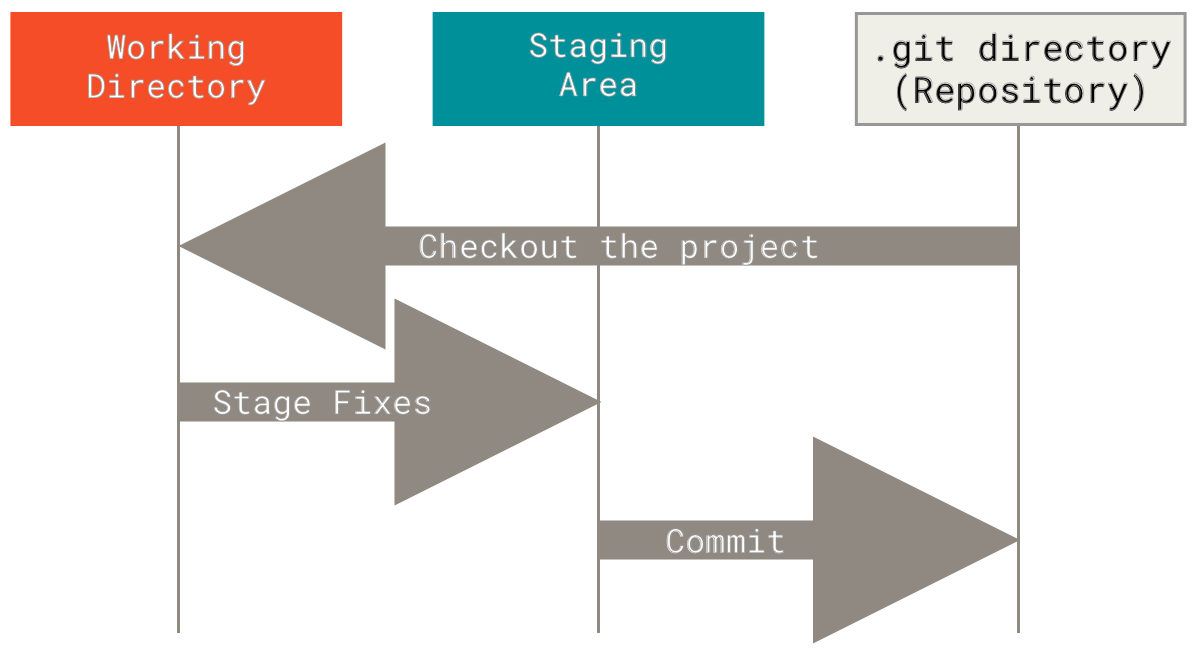
\includegraphics[width=0.8\textwidth]{images/git_file_status.png}
    \caption{Flujo de trabajo en Git}
    \label{fig:git_workflow}
\end{figure}

Estas areas permiten clasificar el estado de los archivos en el proyecto:
\begin{itemize}[leftmargin=*]
  \item \textbf{untracked}: archivo nuevo que Git aún no está siguiendo;
  \item \textbf{modified}: archivo rastreado que fue modificado en el directorio de trabajo, pero todavía no fue agregado al área de preparación;
  \item \textbf{staged}: archivo cuyos cambios fueron agregados al \textbf{staging area} y quedarán incluidos en el próximo commit;
  \item \textbf{committed}: cambios almacenados permanentemente en el repositorio local como parte del historial.
\end{itemize}

Además, al colaborar suele aparecer un \textbf{remote repository} (por ejemplo en GitHub), que es la copia alojada en un servidor
para compartir cambios con otras personas.

\section{Branch}
Una branch (o rama) en Git es una \textbf{línea de tiempo paralela} dentro de tu proyecto.
Las ramas son utilizadas para desarrollar funcionalidades aisladas unas de otras. La rama main o master
es la rama ''por defecto'' cuando creas un repositorio, y es donde se encuentra la \textbf{versión estable del código}.

Durante el desarrollo, es común crear ramas para trabajar en nuevas características, corregir errores
o experimentar sin afectar la rama principal. Este enfoque es útil a la hora de trabajar
colaborativamente, ya que cada desarrollador puede tener su propia rama para sus cambios, evitando modificar
el código sobre el que alguien más está trabajando.

Cada rama es esencialmente una referencia o puntero a un commit específico en la historia del proyecto.
Cuando haces un commit en esa rama, el puntero se mueve hacia adelante, estando siempre apuntando al
último commit de esa línea de desarrollo.

\begin{figure}[h]
  \centering
  \begin{tikzpicture}[scale=1.5, transform shape]
    % Commit DAG
    \gitDAG[grow right sep = 2em]{
      A -- B -- { 
        C,
        D -- E,
      }
    };
    % main branch
    \gitbranch
      {master}     % node name and text 
      {right=of C} % node placement
      {C}          % target
    % HEAD reference
    \gitbranch
      {devel}     % node name and text 
      {right=of E} % node placement
      {E}          % target
  \end{tikzpicture}
  \caption{Ejemplo de ramas en Git}
  \label{fig:git_branches}
\end{figure}

En la figura~\ref{fig:git_branches} se muestra una rama principal (master) que avanza con los commits
A, B y C, mientras que una rama de desarrollo (devel) se bifurca en D y E. Cada rama apunta al último
commit de su línea de desarrollo.

\section{Puntero HEAD}
Git utiliza un puntero llamado HEAD para \textbf{indicar en qué lugar del árbol estás parado actualmente}.
Normalmente HEAD apunta a la rama activa, lo que significa que cualquier commit que hagas se agregará a esa rama.

\begin{figure}[h]
  \centering
  \begin{tikzpicture}[scale=1.5, transform shape]
    % Commit DAG
    \gitDAG[grow right sep = 2em]{
      A -- B -- { 
        C,
        D -- E,
      }
    };
    % main branch
    \gitbranch
      {master}     % node name and text 
      {right=of C} % node placement
      {C}          % target
    % HEAD reference
    \gitbranch
      {devel}     % node name and text 
      {right=of E} % node placement
      {E}          % target
    \gitHEAD
      {above=of master} % node placement
      {master}       % target
  \end{tikzpicture}
  \caption{Puntero HEAD apuntando a la rama master}
  \label{fig:git_head_master}
\end{figure}

En la figura~\ref{fig:git_head_master} se muestra el puntero HEAD apuntando a la rama master, lo que indica
que estamos trabajando en esa rama. Si hacemos un commit, se agregará despues de C, avanzando la rama master.

Es posible apuntar HEAD a un commit específico, este estado se llama ''detached HEAD'' y es útil para revisar versiones anteriores,
pero no nos permite hacer commits permanentes sin crear una nueva rama.

\begin{figure}[h]
  \centering
  \begin{tikzpicture}[scale=1.5, transform shape]
    % Commit DAG
    \gitDAG[grow right sep = 2em]{
      A -- B -- { 
        C,
        D -- E,
      }
    };
    % main branch
    \gitbranch
      {master}     % node name and text 
      {right=of C} % node placement
      {C}          % target
    % HEAD reference
    \gitbranch
      {devel}     % node name and text 
      {right=of E} % node placement
      {E}          % target
    \gitHEAD
      {above=of B} % node placement
      {B}       % target
  \end{tikzpicture}
  \caption{Puntero HEAD apuntando al commit B (detached HEAD)}
  \label{fig:git_head_B}
\end{figure}

En la figura~\ref{fig:git_head_B} se muestra el puntero HEAD apuntando al commit B, lo que indica que estamos
en un estado de detached HEAD. En este estado no deben hacerse commits, ya que no estarán asociados a ninguna
rama y podrían perderse fácilmente.

Veremos que el comando \texttt{git checkout} se usa para cambiar de rama o para moverse a un commit específico, lo que no es mas que
mover el puntero HEAD.

\section{Merge}

\textbf{Merge} significa unir dos ramas.
Existen dos formas de hacer un merge.

\begin{itemize}
  \item \textbf{Fast-forward} (avance rápido):
    Si la rama de destino no tiene nuevos commits desde que se creo la rama que queremos unir (las
    ramas no se han separado), Git simplemente mueve el puntero de la rama de destino hacia adelante,
    apuntando al mismo commit que la rama que estamos uniendo. En este caso, no se crea un nuevo
    commit de merge y la historia es se mantiene lineal.
  \item \textbf{No-fast-forward} (sin avance rápido):
    Si ambas ramas avanzaron por separado, Git crea un nuevo commit especial que tiene dos ''padres'' el último
    commit de cada rama. Es la unión real de las dos historias.
\end{itemize}

Por defecto, git intentará realizar un merge fast-forward.

Al realizar un merge, es posible que surja un conflicto: esto se da si las dos ramas modificaron
el mismo fragmento del mismo archivo de formas distintas, Git no sabe cuál versión conservar y te
pide que lo resuelvas a mano. Ya sea eligiendo una de las dos versiones, o combinandolas.

\chapter{Usando git en la práctica}

\section{Instalación}

\section{Configuración inicial}

\section{Como obtener ayuda}
Para buscar ayuda rápida de comandos:
\begin{itemize}[leftmargin=*]
  \item \texttt{git help <comando>} (ejemplo: \texttt{git help commit});
  \item \texttt{git <comando> -{}-help};
  \item \texttt{git <comando> -h} para ver un resumen corto de opciones.
\end{itemize}

\section{Creando mi primer repositorio}
%comandos git init, git add, git commit, git status, git log.
%ver el historial

\section{Subir repositorio a github}
%crear clave ssh
%crear repositorio en github.
%vincular repositorio local con remoto

\section{workflow}
%git pull, git push, git fetch, git merge

%crear ramas, cambiar de rama, eliminar ramas, comparar ramas, resolver conflictos.


\end{document}